\section{Method}\label{method}

Our method builds on the architecture described in R-CNN.

{[}FIGURE: R-CNN schematic, for contrast with the next figure{]}

\subsection{Dense region evaluation}\label{dense-region-evaluation}

\begin{itemize}
\itemsep1pt\parskip0pt\parsep0pt
\item
  Explain the difference between cropping pixels and cropping
  \texttt{pool5}.
\item
  Explain design choices (single vs multi scale, finding nearest window,
  warping.
\item
  {[}FIGURE: dense region evaluation: multi-scale pyramid, warping{]}
\end{itemize}

\subsection{Cascaded CNN}\label{cascaded-cnn}

\begin{itemize}
\itemsep1pt\parskip0pt\parsep0pt
\item
  Explain the reject option in the CNN evaluation
\item
  Each rejector is trained to distiguish background regions from
  foreground (object) regions.
\item
  Explain training the thresholds
\item
  {[}FIGURE: Cascaded CNN, showing threshold layers{]}
\end{itemize}

\subsection{Dynamic region selection}\label{dynamic-region-selection}

\begin{itemize}
\itemsep1pt\parskip0pt\parsep0pt
\item
  Explain dynamic selection of region batches
\item
  Explain iterative training procedure
\item
  {[}FIGURE: dynamic region selection loop, updating region features{]}
\end{itemize}

\subsection{Combined system}\label{combined-system}

\begin{itemize}
\itemsep1pt\parskip0pt\parsep0pt
\item
  Explain how the components fit together
\item
  {[}FIGURE: schematic of the parts fitting together{]}
\end{itemize}


\begin{figure}[h!]
\begin{center}
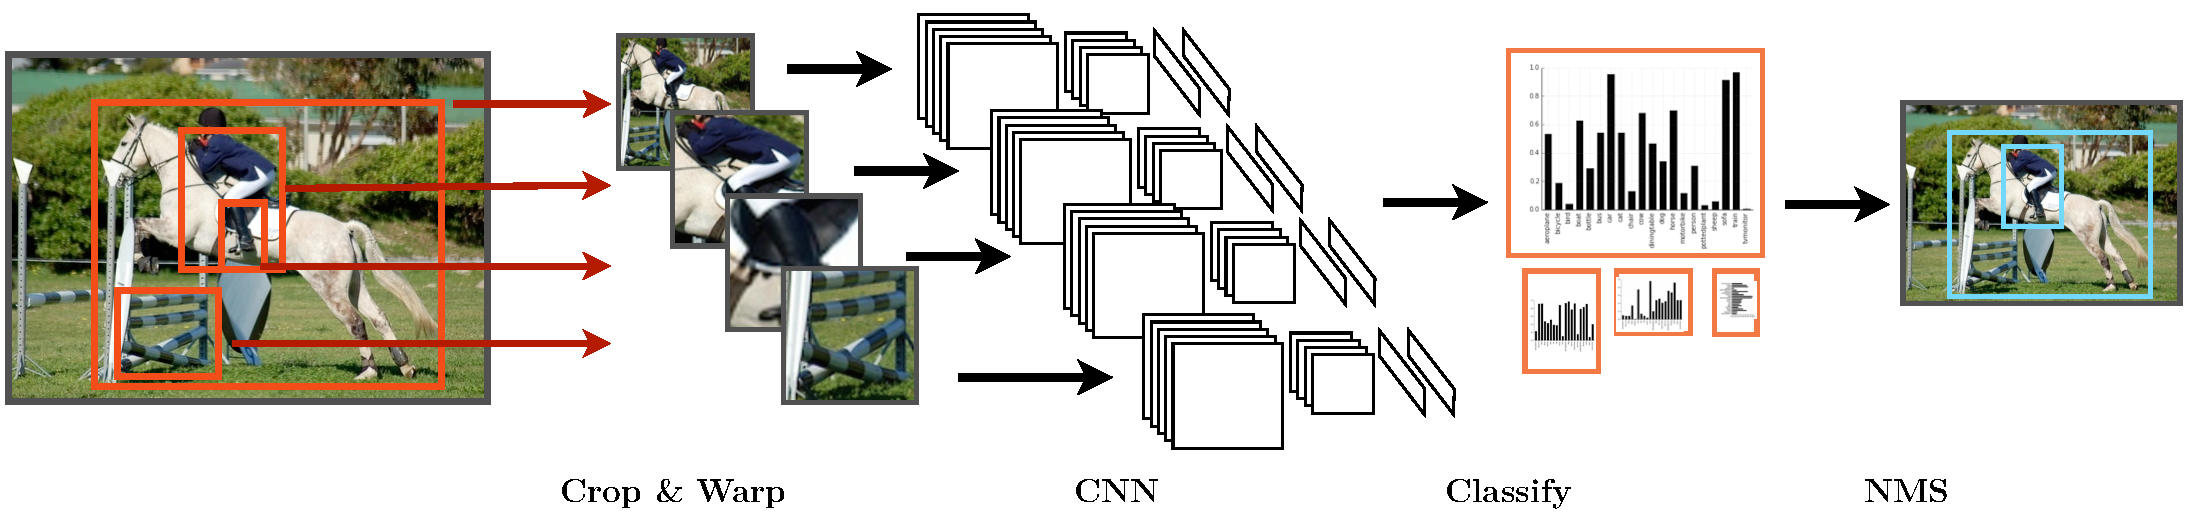
\includegraphics[width=0.98\columnwidth]{figures/rcnn.pdf}
\caption{R-CNN architecture: image regions are cropped, resized, and each one fed
through a CNN with classification layers. The classifier outputs are
post-processed to give the final detections.
}
\end{center}
\end{figure}

\begin{figure}[h!]
\begin{center}
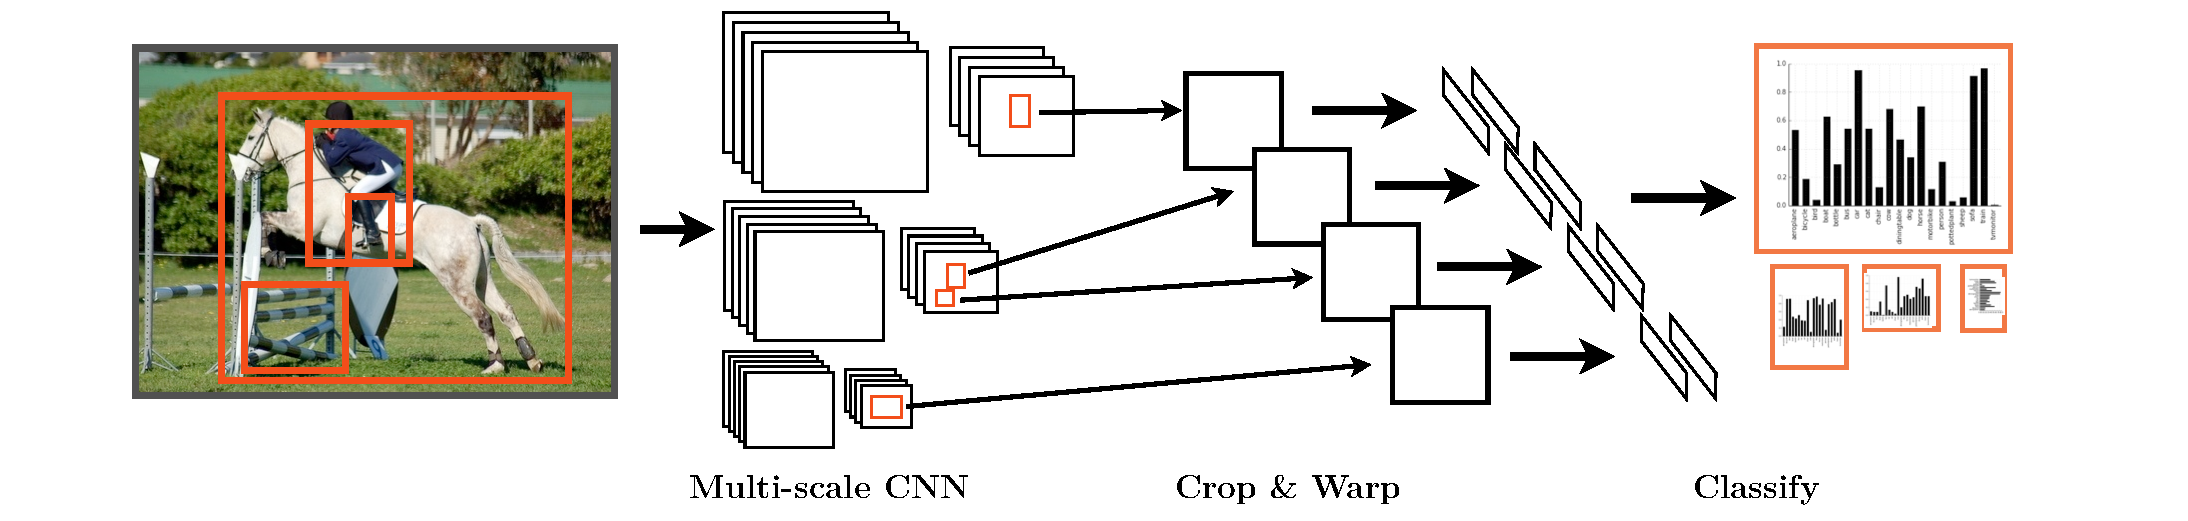
\includegraphics[width=0.98\columnwidth]{figures/dense_rcnn.pdf}
\caption{Dense R-CNN architecture: the whole image is fed through a CNN up to the
highest pooling layer. Regions are cropped from that layer, resized, and
classified. The classifier outputs are post-processed to give the final
detections.
}
\end{center}
\end{figure}
